\subsection{Protocolos de comunicación}
\subsubsection{MQQT}        

MQTT (\textit{Message Queuing Telemetry Transport}) es un protocolo de comunicación ligero diseñado específicamente para entornos con limitaciones de ancho de banda, latencia o recursos, lo que lo hace ideal para aplicaciones de IoT. Desarrollado por IBM en 1999 \cite{mqtt_ibm}, MQTT sigue el modelo \textit{publish/subscribe}, lo que permite la transmisión eficiente de mensajes entre dispositivos conectados sin necesidad de una conexión constante y directa entre ellos. \\


El protocolo MQTT utiliza una arquitectura basada en los siguientes componentes clave que se pueden visualizar su interacción en la figura \ref{fig:mqtt}:

\begin{itemize}
    \item \textbf{\textit{Broker}}: es el servidor central que gestiona la recepción y distribución de los mensajes. El \textit{broker} es responsable de recibir los mensajes de los \textit{publishers} y reenviarlos a los \textit{subscribers} que se hayan suscrito al tema correspondiente.

    \item \textbf{\textit{Publisher}}: es el dispositivo o cliente que envía un mensaje a un tema específico, sin necesidad de conocer a los destinatarios. Solo necesita enviar el mensaje al \textit{broker}.

    \item \textbf{\textit{Subscriber}}: es el dispositivo o cliente que recibe los mensajes de un tema al cual se ha suscrito previamente. El suscriptor se comunica únicamente con el \textit{broker} y no directamente con los publicadores.

    \item  \textbf{\textit{Topics}}: los \textit{topics} o temas son etiquetas jerárquicas utilizadas para categorizar los mensajes en MQTT. Cuando un publicador envía un mensaje, lo asocia con un tema específico. Los suscriptores que se suscriben a ese tema recibirán los mensajes. La flexibilidad de los \textit{topics} permite organizar la información de manera eficiente y estructurada.
\end{itemize}

\begin{figure}[H]
    \centering
    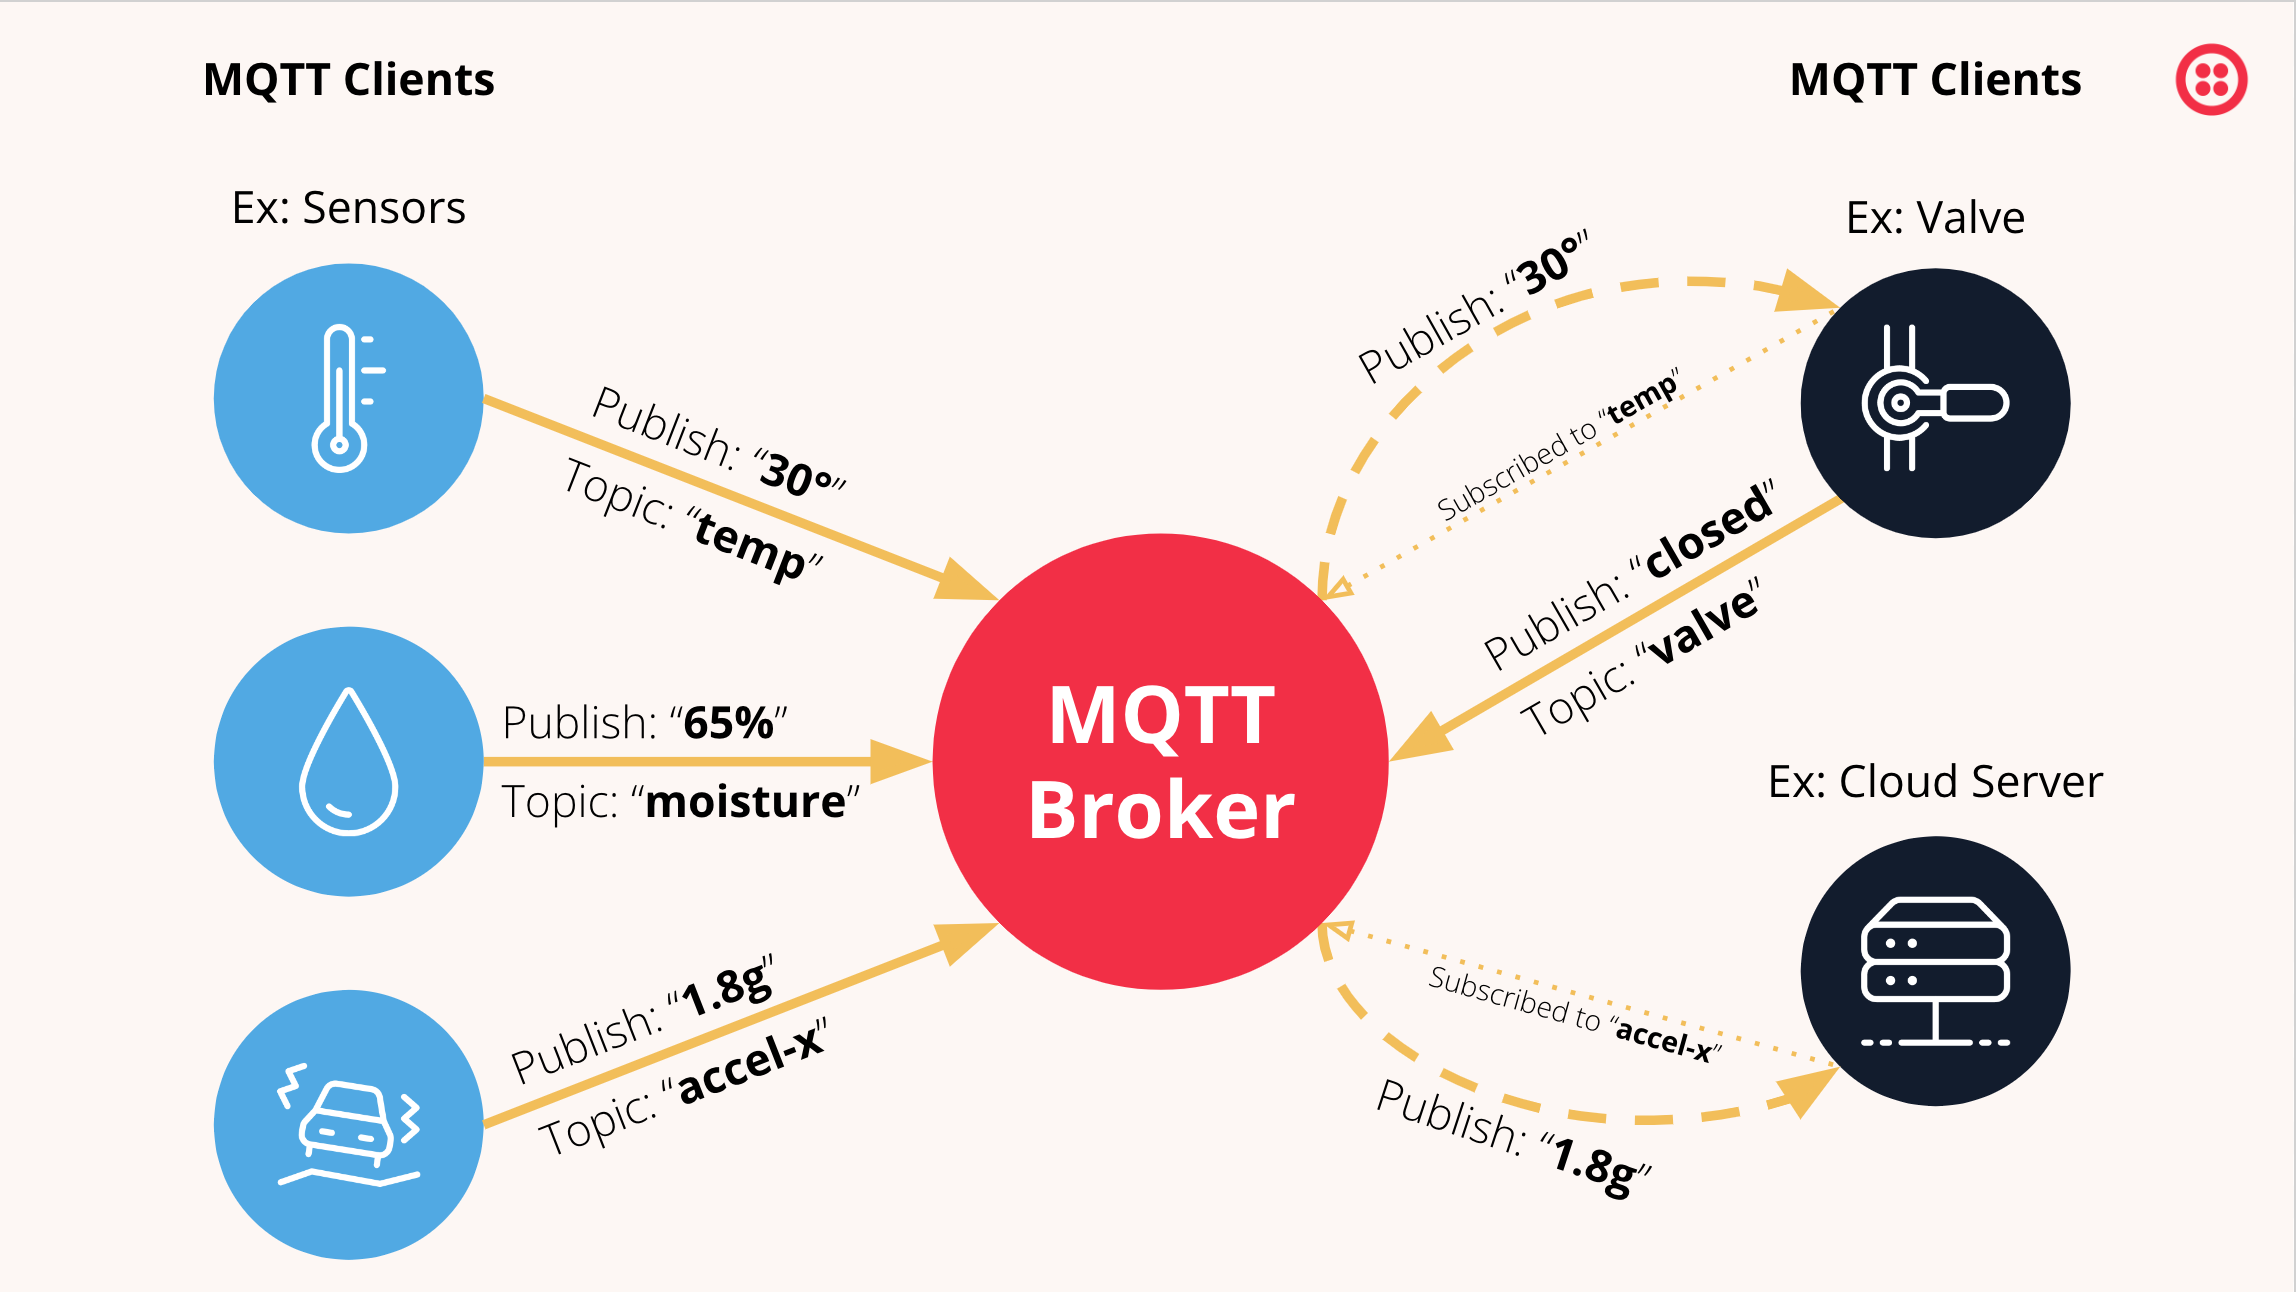
\includegraphics[width = 0.8 \linewidth]{img/mqtt.png}
    \caption{Diagrama de conexión MQTT de ejemplo \cite{mqtt_img}}
    \label{fig:mqtt}
\end{figure}



Las principales ventajas del protocolo MQTT se pueden resumir en:

\begin{itemize}
    \item \textbf{Ligereza}: MQTT está diseñado para ser extremadamente eficiente en cuanto a recursos, lo que lo hace ideal para dispositivos con capacidades limitadas, como sensores o microcontroladores.
    \item \textbf{Minimización del consumo de energía}: al ser un protocolo que no requiere mantener conexiones activas todo el tiempo, los dispositivos pueden ahorrar energía, lo que es fundamental en aplicaciones IoT.
    \item \textbf{Comunicación asíncrona}: gracias a su modelo de publicación y suscripción, los dispositivos no necesitan estar conectados constantemente. El \textit{broker} gestiona las comunicaciones y distribuye los mensajes a los suscriptores según sea necesario.
\end{itemize}



MQTT es ampliamente utilizado en aplicaciones IoT, como monitoreo remoto, automatización industrial, gestión de energía y sistemas embebidos. También se ha implementado en sistemas de emergencia, control de dispositivos y telemetría, donde la eficiencia y la fiabilidad son esenciales.